\documentclass[twocolumn]{iopjournal}

\usepackage{amsmath,amssymb,amsfonts}
\usepackage{graphicx}

\fancyhfoffset[L]{0mm}
\setlength{\marginparwidth}{0pt}
\setlength{\marginparsep}{0pt}
\renewcommand{\dbltopfraction}{0.95}
\renewcommand{\topfraction}{0.95}
\renewcommand{\dblfloatpagefraction}{0.85}

\renewcommand{\articletype}[1]{%
  {\vspace*{-8mm}\noindent \Large \sf Preprint}\par
  \vspace*{6mm}\noindent{\scriptsize \sf{\bfseries \MakeUppercase{#1}}}}

\fancyhead[L]{}
\fancyhead[R]{}

\hypersetup{pdftitle={The Sierpinski Blocks of G's Graded Operator Are a Null Rotation}, pdfauthor={Stephen Nelson}, pdfsubject={Gravity Field Dynamics (GFD)}, pdfkeywords={gravitational constant, Sierpinski triangle, Walsh-Hadamard transform, null rotation, Lorentz group, coupling polynomial, proof}}

\begin{document}

\articletype{Supplementary Material}

\title{The Sierpi\'nski Blocks of G's Graded Operator Are a Null Rotation}

\author{Stephen Nelson}

\affil{Field Dynamics Research}

\ead{stephen@fielddynamics.org}

\begin{abstract}
Gravity Field Dynamics writes Newton's constant as
$G = \tfrac{17}{13}\,\alpha^{21}\,\hbar c/m_e^2$, read from a graded
operator $M_s$ on blocks of size $1$, $4$ and $16$ whose traces are the
coupling polynomial $f(K,s) = 1 + sK + K^2$. The archive draws the
blocks as Sierpi\'nski triangles, $S_m = A^{\otimes m}$ with
$A = \bigl(\begin{smallmatrix}1&0\\1&1\end{smallmatrix}\bigr)$, on
$m = 0, 2, 4$ bits. $G$ reads only their diagonal. Reading the two bits
of the $4$-block as spinor indices, $A$ acts on $4$-vectors as a null
rotation, and we show exactly what $M_s$ is at each state: at
$s = +1$ (TetA) it is the null rotation acting on scalar, vector and
rank-$2$ tensor; at $s = -1$ (TetB) it is that rotation composed with
the total inversion $-1$, not with spatial parity; at $s = 0$ (the
Field Origin) it is their average, the projection onto the part even
under $-1$. The graded trace is the character $1 + s\chi + \chi^2$ with
$\chi = |\mathrm{Tr}\,A|^2 = 4 = K$; among Lorentz transformations
whose trace is real, $\chi = 4$ only for $\pm1$ and the null
rotations. The Walsh--Hadamard read on the $4$-block is a rotation of
space by $\pi$ and factors as null rotation, boost of rapidity $\ln 2$
with a $\pi$ twist, and reverse null rotation. The Jordan chains split
$16$ into $(5 + 3 + 1 + 1) + (3 + 3)$, the pieces of a metric and of a
$2$-form, and the archive's tetrad frame, read in the same way, is a
Newman--Penrose null tetrad. The results identify the operator $G$ is
read from; they do not derive $G$ or $K$.
\end{abstract}

\keywords{gravitational constant, Sierpi\'nski triangle, Walsh--Hadamard transform, null rotation, Lorentz group, coupling polynomial, proof}

% ----------------------------------------------------------------------

\section*{Setting}

The archive derives $G$ from the graded operator
$I_s = P_0 + sP_1 + P_2$ on blocks of size $1$, $K = 4$ and
$K^2 = 16$, the scalar, vector and tensor parts of the tetrad
equation~\cite{Nelson2026gmatrix}. Its traces are $f(K,s) = 21, 17,
13$ at $s = +1, 0, -1$ (TetA, the Field Origin, TetB), and
$\det(\alpha^{I_s}) = \alpha^{\mathrm{Tr}\,I_s}$ gives
$G = \tfrac{17}{13}\,\alpha^{21}\,\hbar c/m_e^2$. The archive's
diagram of this operator~\cite{Nelson2026gdiagram} draws the three
blocks as Sierpi\'nski triangles, and its account of the cube says
that the blocks ``are'' the Sylvester--Hadamard matrices $H_1$, $H_4$,
$H_{16}$~\cite{Nelson2026pixelated}. We take the diagram's blocks at
face value and determine what they are.

\paragraph{Contributions and prior work.} The spinor--vector
correspondence, null rotations~\cite{PenroseRindler}, the
classification of $SL(2,\mathbb{C})$ by its trace~\cite{Beardon1983},
the Jordan structure of a nilpotent element of
$\mathfrak{sl}_2$~\cite{FultonHarris1991}, null tetrads built from a
spin dyad~\cite{NewmanPenrose1962}, Lucas's theorem~\cite{Lucas1878}
and the triangular factorisation of the Walsh--Hadamard matrix are all
standard, and we claim no novelty for them. What is new is the
identification of these structures with the blocks of $G$'s operator
and with the archive's tetrad frame, and the exact form of $M_s$ at the
three states (Theorem~5). In particular, the TetB sign acts on the
vector block as the total inversion $-1$, not as spatial parity. Write
$A = \bigl(\begin{smallmatrix}1&0\\1&1\end{smallmatrix}\bigr)$,
$H_2 = \bigl(\begin{smallmatrix}1&1\\1&-1\end{smallmatrix}\bigr)$,
$S_m = A^{\otimes m}$, and let $|x|$ be the number of $1$-bits of an
index $x$.

\begin{figure*}[!t]
\centering
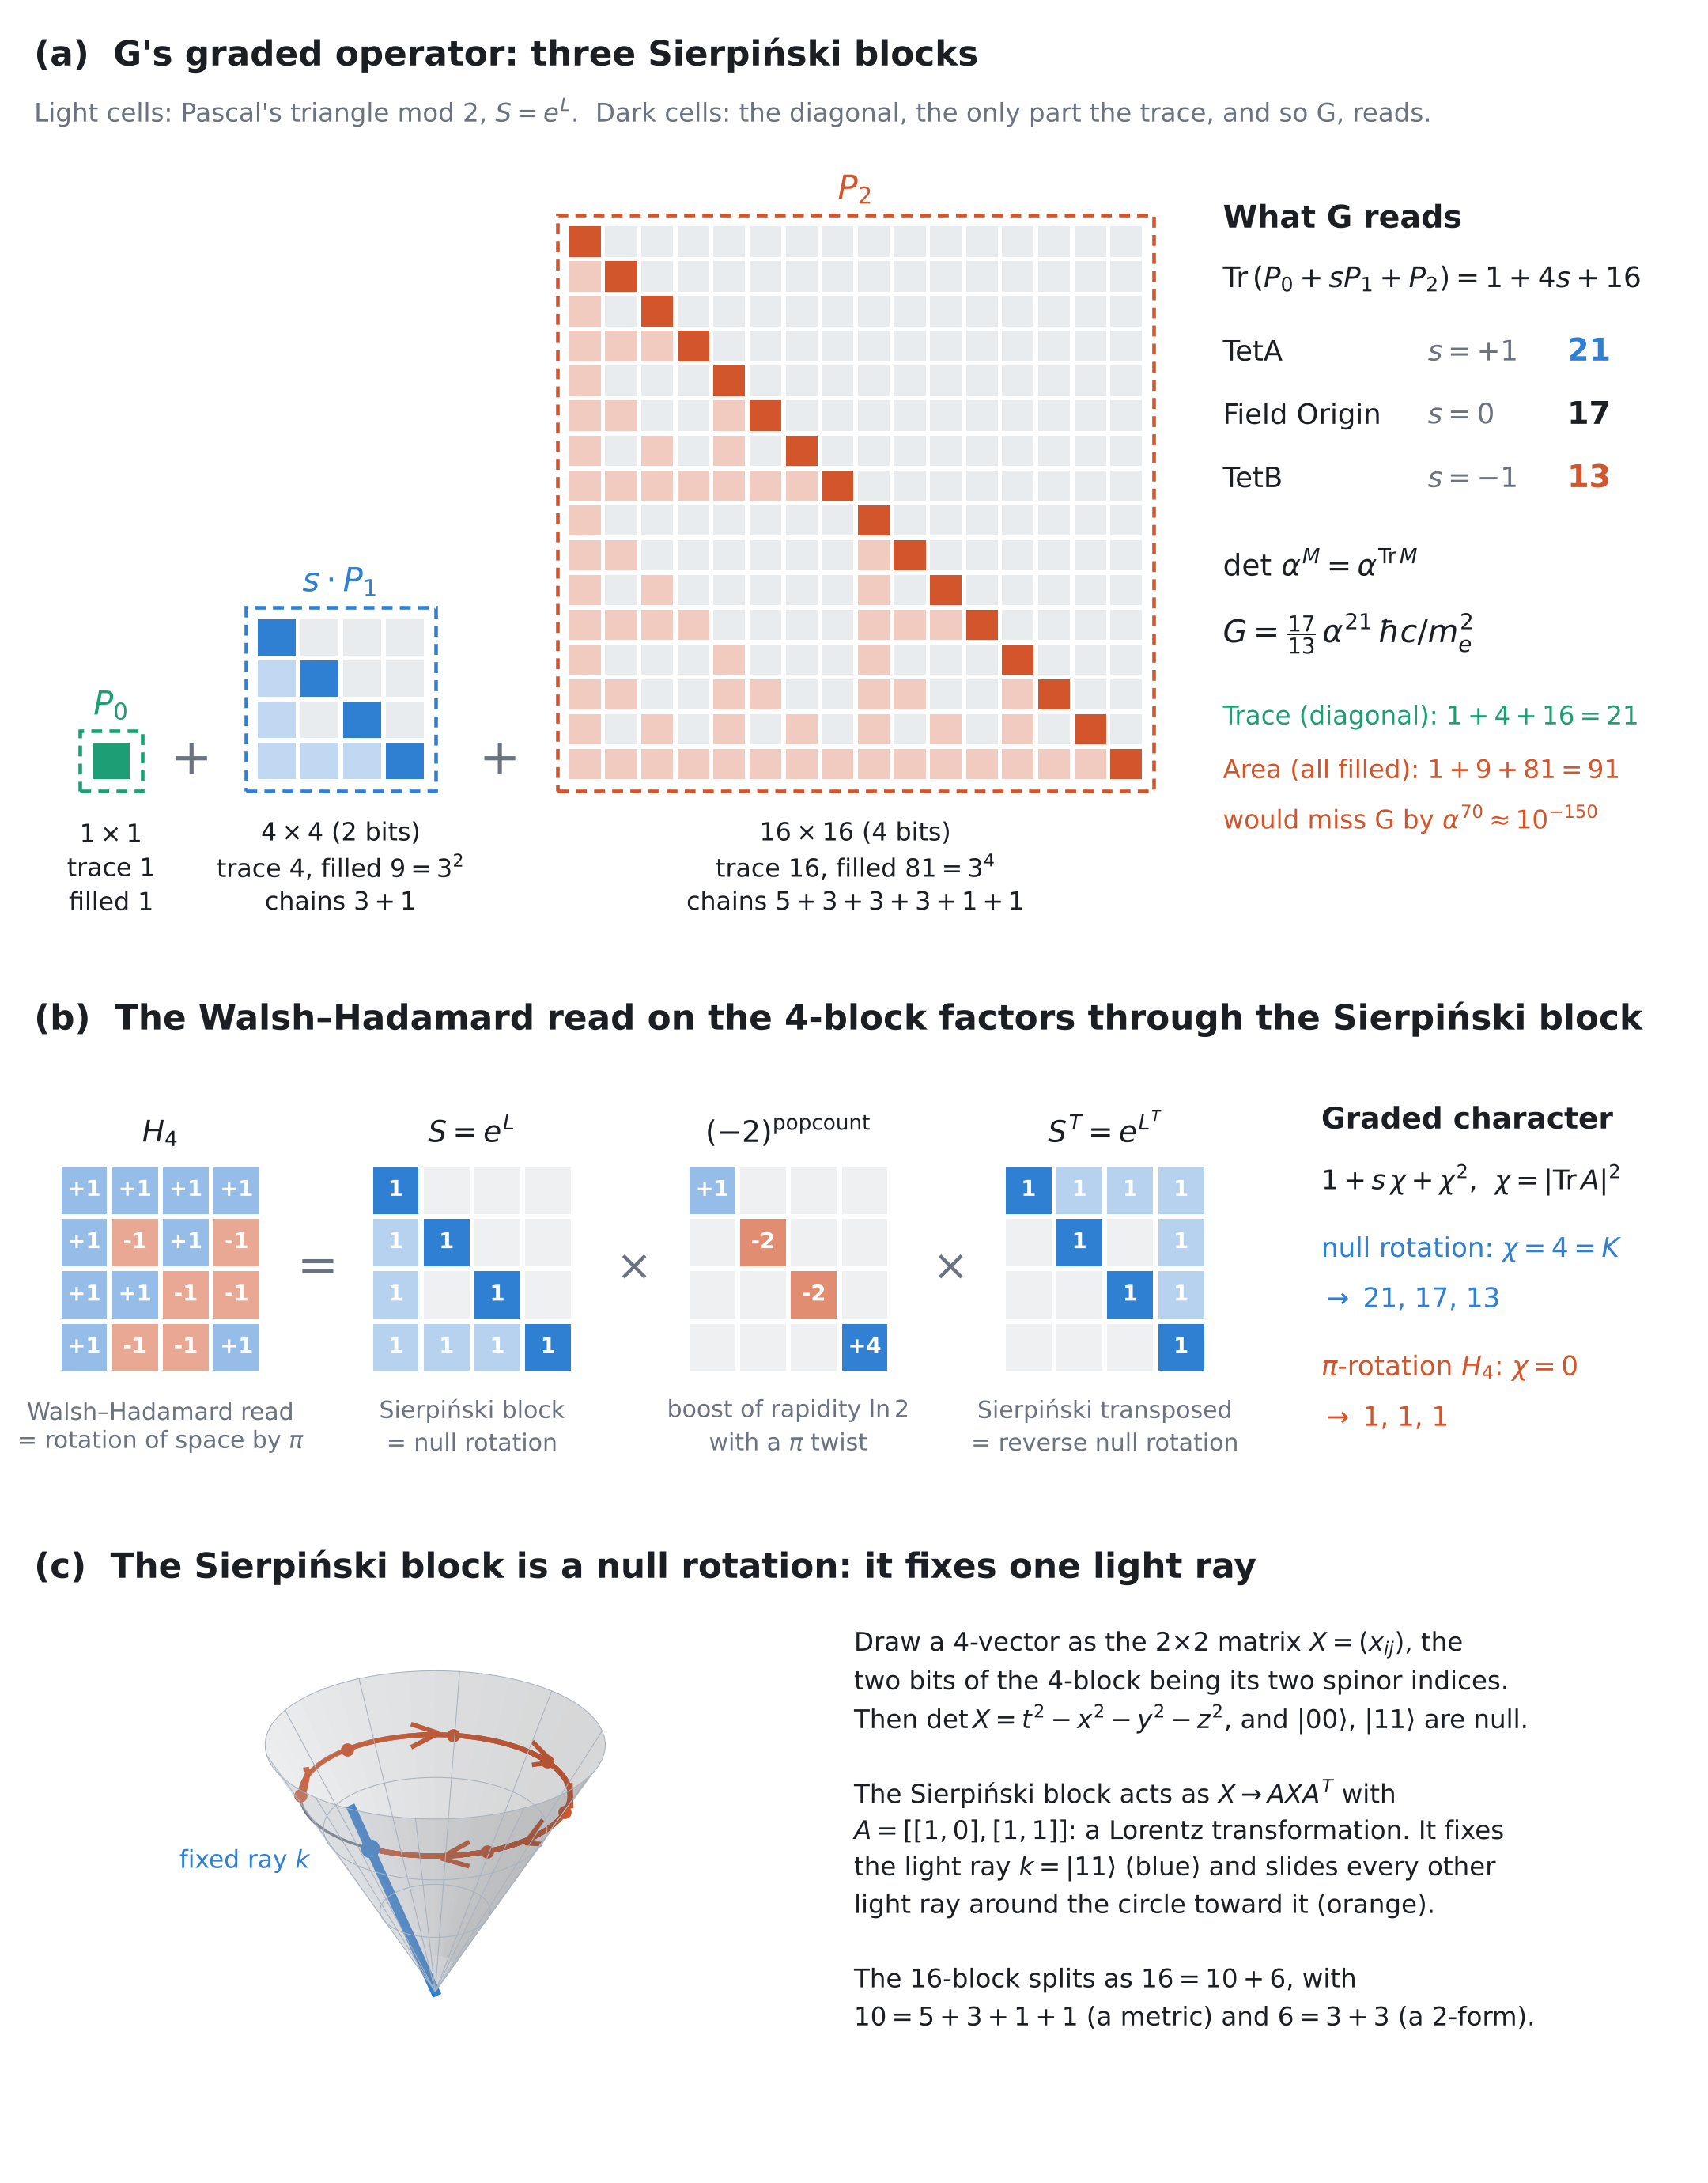
\includegraphics[width=0.8\textwidth]{g_null_rotation_figure.png}
\caption{(a) $G$'s graded operator as drawn in the archive: the
Sierpi\'nski blocks $S_0$, $S_2$, $S_4$. Their diagonals (dark) are all
that the trace, and so $G$, reads. (b) The Walsh--Hadamard read on the
$4$-block factors through the Sierpi\'nski block (Theorem 4).
(c) Read as acting on $4$-vectors, the Sierpi\'nski block fixes the
light ray $|11\rangle$ (Theorem 3); the one-parameter group of null
rotations $A(\tau)$ through it carries every other light ray to it as
$\tau \to \infty$, shown on the slice $y = 0$, which it preserves.}
\label{fig:main}
\end{figure*}

% ----------------------------------------------------------------------

\section*{The Blocks}

\paragraph{Theorem 1 (the Sierpi\'nski blocks).} \textit{The
diagram's blocks are $S_0$, $S_2$ and $S_4$ (checked cell by cell; the
blocks are defined by $S_m = A^{\otimes m}$). Entry $(i,j)$ of $S_m$
is $1$ exactly when the bits of $j$ are a subset of those of $i$,
that is, when $\binom{i}{j}$ is odd. With $L = \sum_{b} N_b$, where
$N_b$ removes bit $b$ (it acts as
$\bigl(\begin{smallmatrix}0&0\\1&0\end{smallmatrix}\bigr)$ on that
bit),}
\begin{equation}
  S_m = e^{L}, \qquad L^{m+1} = 0, \qquad \mathrm{Tr}\,L = 0 .
\end{equation}
\textit{The traces are $1, 4, 16$ and the filled areas are $1, 9,
81 = 3^m$.}

\paragraph{Proof.} The diagram's cells are compared with $S_m$ one by
one. $A = e^{N}$ with $N^2 = 0$, and the $N_b$ commute, so
$A^{\otimes m} = \prod_b e^{N_b} = e^{L}$. The entry rule is the
tensor product of $A$'s and Lucas's theorem. Each bit contributes
$1$ to the trace and $3$ to the area. \hfill $\square$

\paragraph{Theorem 2 ($G$ reads the diagonal).} \textit{Let
$M_s = S_0 \oplus s\,S_2 \oplus S_4$. Then $\mathrm{Tr}\,M_s =
1 + 4s + 16 = f(K,s)$, the spectra of $M_s$ and $I_s$ coincide (rank
$17$ at $s = 0$; $17$ eigenvalues $+1$ and $4$ eigenvalues $-1$ at
$s = -1$), and $\det(\alpha^{M_s}) = \alpha^{f(K,s)}$. So $G$ is the
same whether the blocks are identities or Sierpi\'nski blocks.}

\paragraph{Proof.} Each $S_m$ is lower triangular with unit
diagonal, so its eigenvalues are all $1$. $\det e^{X} =
e^{\mathrm{Tr}\,X}$. \hfill $\square$

\medskip
\noindent
So the Sierpi\'nski structure off the diagonal is invisible to $G$.
For comparison only: reading the filled cells instead,
$1 + 9 + 81 = 91$, would change $G$ by $\alpha^{70} \approx 10^{-150}$.
The next theorems say what the off-diagonal structure is.

% ----------------------------------------------------------------------

\section*{The Lorentz Reading}

Write a $4$-vector as $X = t + x\sigma_1 + y\sigma_2 + z\sigma_3$, so
that $\det X = t^2 - x^2 - y^2 - z^2$, and index its entries by the
two bits of the $4$-block, $X = (x_{ij})$~\cite{PenroseRindler}. The
states $|00\rangle$ and $|11\rangle$ are $t + z$ and $t - z$, the two
null directions along $z$.

\paragraph{Theorem 3 (the Sierpi\'nski block is a null rotation).}
\textit{On the bit basis, $S_2\,\mathrm{vec}(X) = \mathrm{vec}(AXA^T)$.
The map $\Lambda_A : X \mapsto AXA^{\dagger}$ is a proper
orthochronous Lorentz transformation with $\Lambda_A \ne 1$ and
$(\Lambda_A - 1)^3 = 0$: a null rotation. Its fixed vectors form the
plane spanned by $k = (1,0,0,-1)$, the state $|11\rangle$, and the
$y$ axis, and $k$ is the only light ray in that plane. Every real $A$
with $\det A = 1$ fixes $y$, so the Sierpi\'nski blocks act as the
Lorentz group of $(t, x, z)$.}

\paragraph{Proof.} $\mathrm{vec}(AXA^T) = (A \otimes A)\,
\mathrm{vec}(X)$, and $A$ is real, so $A^T = A^\dagger$.
$\det(AXA^\dagger) = \det X$ because $\det A = 1$. $A$ fixes
$|1\rangle$, so $\Lambda_A$ fixes the matrix
$|1\rangle\langle1|$, which is the light ray $k$. The antisymmetric part $y\,i\sigma_2$ is sent to
$\det A \cdot y\,i\sigma_2$. The remaining statements are computed
from the $4 \times 4$ matrix of $\Lambda_A$. \hfill $\square$

\paragraph{Remark (the one-parameter group).} $A(\tau) =
\bigl(\begin{smallmatrix}1&0\\\tau&1\end{smallmatrix}\bigr)$ is the
one-parameter group of null rotations about $k$. A boost along $z$
conjugates it to itself with a new parameter, $B(\eta)A(\tau)B(\eta)^{-1}
= A(\tau e^{-\eta})$, so every $A(\tau)$ with $\tau > 0$ is equivalent
to the Sierpi\'nski block $A(1)$, and the entry $1$ is a convention. As
$\tau \to \infty$, $A(\tau)$ carries every other light ray to $k$.

\paragraph{Theorem 4 (the Hadamard read).} \textit{The normalised
$H_2/\sqrt2$ acts on $4$-vectors as a rotation of space by $\pi$ about
$(\hat x + \hat z)/\sqrt2$. For $m = 0, 2, 4$,}
\begin{equation}
\begin{aligned}
  H_{2^m} &= S_m\,\mathrm{diag}\big((-2)^{|x|}\big)\,S_m^{T}\\
  &= e^{L}\,e^{(\ln 2 + i\pi)|x|}\,e^{L^T}.
\end{aligned}
\end{equation}
\textit{On the $4$-block the middle factor
$\mathrm{diag}(1,-2)/\sqrt2$ is a boost of rapidity $\ln 2$ along $z$
combined with a rotation by $\pi$ about $z$. So the rotation by $\pi$
is a null rotation, a boost with a $\pi$ twist, and the reverse null
rotation.}

\paragraph{Proof.} For one bit,
$A\,\mathrm{diag}(1,-2)\,A^T = H_2$; tensor powers give the rest, and
$(-2)^{|x|} = e^{(\ln 2 + i\pi)|x|}$. The Lorentz matrices follow
from $\Lambda_M = \tfrac12\mathrm{Tr}(\sigma_\mu M \sigma_\nu
M^\dagger)$, with $\cosh\ln2 = \tfrac54$ and $\sinh\ln2 = \tfrac34$.
\hfill $\square$

\medskip
\noindent
This is an elementary triangular factorisation of the Walsh--Hadamard
matrix (the matrix itself is Sylvester's~\cite{Sylvester1867}). In it,
the Sierpi\'nski blocks are the outer factors and the half-turn
$e^{i\pi}$ sits in the middle.

% ----------------------------------------------------------------------

\section*{The Character}

\paragraph{Theorem 5 (the three states, and $K = 4$).} \textit{Let
$\rho(V) = 1 \oplus V \oplus (V \otimes V)$ be the action of a Lorentz
transformation $V$ on scalar, vector and rank-$2$ tensor, and
$\Lambda = A \otimes A$ the Sierpi\'nski block in the bit basis. Then}
\begin{equation}
\begin{aligned}
  M_{+1} &= \rho(\Lambda), \qquad M_{-1} = \rho(-\Lambda),\\
  M_0 &= \tfrac12\big(M_{+1} + M_{-1}\big) = \rho(\Lambda)\,\Pi_+ ,
\end{aligned}
\end{equation}
\textit{where $-1$ is the total inversion (PT), which acts as $-1$ on
vectors and $+1$ on tensors, and $\Pi_+ = \tfrac12(1 + \rho(-1))$ is
the projection onto the part even under it. Spatial parity
$P = \mathrm{diag}(1,-1,-1,-1)$ does not give TetB: the graded trace of
$P\Lambda$ is $1$. For $M \in SL(2,\mathbb{C})$ the trace of $\Lambda_M$
on vectors is $\chi = |\mathrm{Tr}\,M|^2$ and on tensors $\chi^2$, so
$\mathrm{Tr}\,\rho(\pm\Lambda_M) = 1 \pm \chi + \chi^2 = f(\chi, \pm1)$.
The null rotation has $\chi = 4 = K$, giving $21, 17, 13$; the
$\pi$-rotation $H_2/\sqrt2$ has $\chi = 0$. If $\mathrm{Tr}\,M$ is real,
then $\chi = 4$ exactly when $M = \pm1$ or $M$ is a null rotation (up
to sign); $\chi < 4$ for elements conjugate to rotations and $\chi > 4$
for those conjugate to boosts. Elements with non-real trace, which
combine a boost and a rotation, can also have $\chi = 4$.}

\paragraph{Proof.} The blocks of $M_{\pm1}$ are $1$, $\pm(A\otimes A)$
and $(A\otimes A)^{\otimes 2} = S_4$, and $(-1)^{\otimes 2} = +1$ on
tensors. $\Lambda_M$ is $M \otimes \bar M$ in the bit basis, so its
trace is $\mathrm{Tr}\,M\,\overline{\mathrm{Tr}\,M}$, and traces
multiply over tensor products. $\mathrm{Tr}\,A = 2$,
$\mathrm{Tr}\,H_2 = 0$, and $\mathrm{Tr}(P\Lambda_A) = -1$. The
classification by trace is standard~\cite{Beardon1983}: real trace in
$(-2,2)$ is elliptic, $\pm2$ is parabolic or $\pm1$, and real
$|\mathrm{Tr}| > 2$ is hyperbolic. The loxodromic example
$\mathrm{Tr}\,M = 2e^{i\pi/3}$ is in the checks. \hfill $\square$

\medskip
\noindent
This gives $G$'s three traces an exact reading: TetA is the null
rotation on scalar, vector and tensor; TetB adds the total inversion;
the Field Origin is the even projection, which is why
$17 = (21 + 13)/2$. It does not derive $K = 4$, which comes from
$D = 3$~\cite{Nelson2026hadamard}, and the identity has the same
character. It shows that the blocks the archive draws are null
rotations, and that the Walsh--Hadamard read itself, with $\chi = 0$,
could not give $G$'s numbers.

\paragraph{Theorem 6 (the chains).} \textit{The Jordan chains of $S_2$
have lengths $3 + 1$, and those of $S_4$ have lengths $5 + 3 + 3 + 3 +
1 + 1$. They are the Clebsch--Gordan decompositions of $2$ and $4$
spin-$\tfrac12$ factors, and over the whole operator
$21 = 1 + (3 + 1) + (5 + 3 + 3 + 3 + 1 + 1)$. $S_4$ commutes with the
exchange of the two vector factors, and on the symmetric $10$ and
antisymmetric $6$ its chains are}
\begin{equation}
  10 = 5 + 3 + 1 + 1, \qquad 6 = 3 + 3 .
\end{equation}

\paragraph{Proof.} $L$ is the lowering operator of the diagonal
$\mathfrak{sl}_2$ on $m$ spin-$\tfrac12$ factors, so each irreducible
summand of dimension $d$ is one chain of length $d$. The multiplicity
of dimension $m - 2k + 1$ is $\binom{m}{k} - \binom{m}{k-1}$. The
restriction to the symmetric and antisymmetric parts is computed from
the ranks of $(S_4 - 1)^j$. \hfill $\square$

\medskip
\noindent
The split $16 = 10 + 6$ is the archive's: general relativity keeps the
symmetric $10$, and the antisymmetric $6$ is the torsion-type part.
The chains refine it into the pieces of a symmetric tensor
($5 + 3 + 1 + 1$) and of a $2$-form ($3 + 3$).

% ----------------------------------------------------------------------

\section*{The Tetrad Frame}

\paragraph{Theorem 7 (the frame is the $4$-block read).}
\textit{The archive's tetrad frame~\cite{Nelson2026hadamard}, a row of
ones over the four TetA corners $(1,1,1)$, $(1,-1,-1)$, $(-1,1,-1)$,
$(-1,-1,1)$, is $H_2 \otimes H_2$ with its second and third rows
exchanged. So it factors through the Sierpi\'nski block,}
\begin{equation}
  e = P\,S_2\,\mathrm{diag}\big((-2)^{|x|}\big)\,S_2^{T},
\end{equation}
\textit{with $P$ the row exchange: a null rotation, a boost of rapidity
$\ln 2$ with a $\pi$ twist, and the reverse null rotation. Read in
$(t, x, y, z)$, the frame is not a Lorentz structure:
$e^T\eta\,e = 2J - 4I$, which is $J$ minus the archive's forced Gram
matrix $4I - J$.}

\paragraph{Proof.} Direct comparison, and Theorem 4 with $m = 2$.
\hfill $\square$

\medskip
\noindent
So the same $4 \times 4$ matrix plays two roles. As an operator on the
$4$-block it is a Lorentz transformation, the rotation by $\pi$. As a
set of four legs it is the frame. The next theorem reads the legs in
the spinor picture.

\paragraph{Theorem 8 (a Newman--Penrose null tetrad).} \textit{Read
with its two bits as spinor indices, leg $(a, b)$ of
$H_2 \otimes H_2$ is the matrix $X = h_a h_b^T$, with $h_0, h_1$ the
columns of $H_2$, so every leg has $\det X = 0$. In Minkowski
components}
\begin{equation}
\begin{aligned}
  l &= (1, 1, 0, 0), & n &= (1, -1, 0, 0),\\
  m &= (0, 0, -i, 1), & \bar m &= (0, 0, i, 1),
\end{aligned}
\end{equation}
\textit{with $l\cdot n = 2$, $m\cdot\bar m = -2$ and every other
product $0$: a Newman--Penrose null
tetrad~\cite{NewmanPenrose1962}, built from the spinor dyad
$(h_0, h_1)$, whose normalisation $\varepsilon(h_0, h_1) = -2$
accounts for the factor $2$. Its Hadamard combinations $l \pm n$, $m + \bar m$ and
$i(m - \bar m)$ are $2t$, $2x$, $2z$ and $2y$. In any spinor reading,
$X \mapsto BXC^T$ with $B$, $C$ invertible, at most two of the four
legs are real light rays.}

\paragraph{Proof.} The column $(a, b)$ of $H_2 \otimes H_2$ is
$h_a \otimes h_b = \mathrm{vec}(h_a h_b^T)$, a matrix of rank one.
The components and products follow from
$x^\mu = \tfrac12\mathrm{Tr}(\sigma_\mu X)$ and the polarisation of
$\det$. For the bound: a rank-one matrix $pq^T$ is Hermitian exactly
when $q$ is a real multiple of $\bar p$. If the legs $(a,0)$ and
$(a,1)$ were both Hermitian, then $Ch_0$ and $Ch_1$ would both be
multiples of $\overline{Bh_a}$, which is impossible for invertible
$C$. So each $a$ contributes at most one real light ray.
\hfill $\square$

\medskip
\noindent
So the frame's four legs are null in the spinor picture, in the form
general relativity uses for null tetrads: two real light rays and one
complex-conjugate pair. This is a different reading from Letter~1's.
There the legs are $(1, v/\sqrt3)$, the Hadamard frame with its
spatial rows rescaled by $1/\sqrt3$, and all four are real light rays
on the celestial sphere. Both readings make the frame null; they
differ in which coordinates carry the two bits.

% ----------------------------------------------------------------------

\section*{Scope}

The results are exact. They identify the operator from which $G$ is
read; they do not derive $G$. The operator is a null rotation only at
TetA; TetB composes it with the total inversion $-1$, and the Field
Origin is a projection, not a Lorentz transformation. That the TetB
sign acts on the vector block as PT, rather than as the spatial parity
that exchanges TetA and TetB in three dimensions, is an open point for
the framework's reading of the two chambers. The value of $G$ still rests on the
archive's assumption that each of the $21$ coupling levels contributes
one factor of $\alpha$~\cite{Nelson2026gmatrix}, and on $K = 4$ from
$D = 3$. The trace cannot tell a null rotation from the identity, so
the content added here is what the blocks are: Sierpi\'nski triangles,
null rotations, and the outer factors of the Walsh--Hadamard read. The
statement that the blocks ``are'' $H_1$, $H_4$, $H_{16}$ is sharpened
accordingly: they are the Sierpi\'nski factors of those matrices, and
the matrices themselves have trace $0$ beyond $H_1$. The Sierpi\'nski
blocks act through the Lorentz group of $(t, x, z)$, with $y$ fixed.
So the chain lengths match the decomposition of a vector, a metric and
a $2$-form exactly, but naming the components ($h_{00}$, $h_{0i}$,
\dots) requires the rotation group, which the Sierpi\'nski block does
not supply. The spinor--vector correspondence, null rotations and the
factorisation of the Hadamard matrix are standard, as is the
construction of a null tetrad from a spinor dyad; the identification
with $G$'s blocks and with the archive's tetrad frame is new. Theorem 8
gives two real null legs, not four, in the spinor reading. The
Hadamard frame read directly in $(t, x, y, z)$ has legs of norm $-2$;
rescaling its spatial rows by $1/\sqrt3$, as Letter~1 does, makes all
four legs real light rays.

% ----------------------------------------------------------------------

\begin{thebibliography}{99}

\bibitem{Nelson2026gmatrix}
S.~Nelson,
\textit{G as a matrix read} (2026), research archive,
\texttt{g\_from\_topology/g\_matrix\_synthesis.md}.

\bibitem{Nelson2026gdiagram}
S.~Nelson,
\textit{G as three Sierpi\'nski blocks} (2026), research archive,
\texttt{g\_from\_topology/}\linebreak\texttt{g\_three\_sierpinski\_blocks.html}.

\bibitem{Nelson2026pixelated}
S.~Nelson,
\textit{The universe is pixelated} (2026), research archive,
\texttt{universe-is-pixelated/}.

\bibitem{Nelson2026hadamard}
S.~Nelson,
\textit{The Stellated Octahedron, the Cube and the Hadamard Matrix}
(2026).

\bibitem{PenroseRindler}
R.~Penrose and W.~Rindler,
\textit{Spinors and Space-Time}, vol.~1
(Cambridge University Press, 1984).

\bibitem{NewmanPenrose1962}
E.~Newman and R.~Penrose,
``An approach to gravitational radiation by a method of spin
coefficients'', \textit{J. Math. Phys.} \textbf{3} (1962) 566--578.

\bibitem{Lucas1878}
E.~Lucas,
``Th\'eorie des fonctions num\'eriques simplement p\'eriodiques'',
\textit{Amer. J. Math.} \textbf{1} (1878) 184--240, 289--321.

\bibitem{FultonHarris1991}
W.~Fulton and J.~Harris,
\textit{Representation Theory: A First Course}
(Springer, New York, 1991).

\bibitem{Beardon1983}
A.~F.~Beardon,
\textit{The Geometry of Discrete Groups}
(Springer, New York, 1983).

\bibitem{Sylvester1867}
J.~J.~Sylvester,
``Thoughts on inverse orthogonal matrices'',
\textit{Phil. Mag.} \textbf{34} (1867) 461--475.

\end{thebibliography}

\end{document}
